% =============================================================================
%  AAKASHVANI CanSat — User Manual
%  Build:  xelatex user_manual.tex   (run twice for the table of contents)
%          or: latexmk -xelatex user_manual.tex
%  Fonts:  IBM Plex (SIL OFL), loaded from ../../tools/assets/fonts/
% =============================================================================
\documentclass[11pt,a4paper,oneside]{article}

\usepackage[a4paper,margin=22mm,top=24mm,bottom=24mm,headheight=14pt]{geometry}
\usepackage{fontspec}
\usepackage{xcolor}
\usepackage{graphicx}
\usepackage{tikz}
\usetikzlibrary{arrows.meta,positioning,calc}
\usepackage[most]{tcolorbox}
\usepackage{enumitem}
\usepackage{booktabs}
\usepackage{tabularx}
\usepackage{array}
\usepackage{fancyhdr}
\usepackage{titlesec}
\usepackage{float}
\usepackage{needspace}
\usepackage[hidelinks]{hyperref}

% ----------------------------------------------------------------- fonts
\defaultfontfeatures{Ligatures=TeX}
\setmainfont{IBMPlexSans}[
  Path=../../tools/assets/fonts/, Extension=.ttf,
  UprightFont=*-Regular, BoldFont=*-SemiBold,
  ItalicFont=*-Regular, ItalicFeatures={FakeSlant=0.18},
  BoldItalicFont=*-SemiBold, BoldItalicFeatures={FakeSlant=0.18}]
\setmonofont{IBMPlexMono}[
  Path=../../tools/assets/fonts/, Extension=.ttf,
  UprightFont=*-Regular, BoldFont=*-SemiBold, Scale=0.92]
\newfontfamily\headfont{IBMPlexSans}[
  Path=../../tools/assets/fonts/, Extension=.ttf, UprightFont=*-Bold]

% ----------------------------------------------------------------- colours
\definecolor{ink}{HTML}{1B2129}
\definecolor{muted}{HTML}{5B6573}
\definecolor{accent}{HTML}{C98410}
\definecolor{accentbg}{HTML}{FFF5E3}
\definecolor{okbg}{HTML}{E8F6EE}
\definecolor{okfg}{HTML}{1F7A47}
\definecolor{warnbg}{HTML}{FDECEC}
\definecolor{warnfg}{HTML}{B3261E}
\definecolor{rule}{HTML}{D9DEE5}
\definecolor{panel}{HTML}{F4F6F9}
% LED colours
\definecolor{ledwhite}{HTML}{E6E6E6}
\definecolor{ledblue}{HTML}{1E5BD8}
\definecolor{ledviolet}{HTML}{8A3FD1}
\definecolor{ledgreen}{HTML}{16A34A}
\definecolor{ledamber}{HTML}{F59E0B}
\definecolor{ledred}{HTML}{DC2626}
\definecolor{ledmagenta}{HTML}{D61FAE}
\definecolor{ledorange}{HTML}{F97316}
\definecolor{ledpurple}{HTML}{A21CAF}
\definecolor{ledcyan}{HTML}{06B6D4}
\color{ink}

% ----------------------------------------------------------------- layout helpers
\setlength{\parindent}{0pt}
\setlength{\parskip}{6pt}
\linespread{1.12}
\setlist{itemsep=3pt,topsep=4pt,leftmargin=*}
\setlist[enumerate]{label=\textbf{\arabic*.}}

\titleformat{\section}{\needspace{9\baselineskip}\headfont\Large\color{ink}}{\color{accent}\thesection}{0.7em}{}[\vspace{-4pt}{\color{rule}\rule{\linewidth}{0.6pt}}]
\titleformat{\subsection}{\needspace{6\baselineskip}\headfont\large\color{ink}}{\color{accent}\thesubsection}{0.6em}{}
\titlespacing*{\section}{0pt}{18pt}{8pt}
\titlespacing*{\subsection}{0pt}{12pt}{4pt}

\pagestyle{fancy}
\fancyhf{}
\fancyhead[L]{\small\color{muted}Aakashvani CanSat · User Manual}
\fancyhead[R]{\small\color{muted}Team 001}
\fancyfoot[C]{\small\color{muted}\thepage}
\renewcommand{\headrulewidth}{0pt}

\newcommand{\led}[1]{\tikz[baseline=-0.65ex]{\fill[#1] (0,0) circle (1.05ex); \draw[black!35,line width=0.3pt] (0,0) circle (1.05ex);}}
\newcommand{\btn}[1]{\tikz[baseline=(b.base)]\node[draw=rule,fill=panel,rounded corners=2pt,inner xsep=4pt,inner ysep=2pt,font=\small](b){#1};}
\newcommand{\page}[1]{\textbf{#1}}
\newcommand{\cmd}[1]{\texttt{#1}}
\newcommand{\judgesfile}{\texttt{Documents\textbackslash\allowbreak Aakashvani\textbackslash\allowbreak Flight\_2026-IN-SPACeCAN-7USAT-001.csv}}

\newtcolorbox{tip}[1][Tip]{enhanced,breakable,colback=accentbg,colframe=accentbg,coltitle=accent,
  fonttitle=\bfseries,title=#1,attach title to upper={\ \ },boxrule=0pt,arc=3pt,left=8pt,right=8pt,top=6pt,bottom=6pt,
  borderline west={3pt}{0pt}{accent}}
\newtcolorbox{danger}[1][Safety]{enhanced,breakable,colback=warnbg,colframe=warnbg,coltitle=warnfg,
  fonttitle=\bfseries,title=#1,attach title to upper={\ \ },boxrule=0pt,arc=3pt,left=8pt,right=8pt,top=6pt,bottom=6pt,
  borderline west={3pt}{0pt}{warnfg}}
\newtcolorbox{good}[1][Good to know]{enhanced,breakable,colback=okbg,colframe=okbg,coltitle=okfg,
  fonttitle=\bfseries,title=#1,attach title to upper={\ \ },boxrule=0pt,arc=3pt,left=8pt,right=8pt,top=6pt,bottom=6pt,
  borderline west={3pt}{0pt}{okfg}}

\newcommand{\shot}[3][\linewidth]{%
  \begin{figure}[H]\centering
  \tcbox[enhanced,colback=white,colframe=rule,boxrule=0.5pt,arc=3pt,left=0pt,right=0pt,top=0pt,bottom=0pt]{\includegraphics[width=#1]{img/#2}}
  \par\vspace{2pt}{\small\color{muted}#3}
  \end{figure}}

\newcolumntype{L}{>{\raggedright\arraybackslash}X}

% =============================================================================
\begin{document}

% ----------------------------------------------------------------- cover
\begin{titlepage}
\thispagestyle{empty}
\begin{tikzpicture}[remember picture,overlay]
  \fill[ink] (current page.north west) rectangle ([yshift=-11cm]current page.north east);
  \fill[accent] ([yshift=-11cm]current page.north west) rectangle ([yshift=-11.25cm]current page.north east);
  % flight path sketch
  \draw[white!35,line width=0.8pt,dashed] ([xshift=11.5cm,yshift=-9.6cm]current page.north west)
     .. controls +(0.6,4.6) and +(-1.2,0.2) .. ([xshift=14cm,yshift=-3.2cm]current page.north west)
     .. controls +(1.2,-0.2) and +(0,2.5) .. ([xshift=16.8cm,yshift=-7.2cm]current page.north west)
     .. controls +(-0.2,-1.4) and +(1.4,0) .. ([xshift=13.6cm,yshift=-9.6cm]current page.north west);
  \fill[accent] ([xshift=14cm,yshift=-3.2cm]current page.north west) circle (2.2pt);
  \fill[white] ([xshift=13.6cm,yshift=-9.6cm]current page.north west) circle (2.2pt);
  \node[anchor=north west,text=white,align=left] at ([xshift=2.2cm,yshift=-2.6cm]current page.north west)
    {{\headfont\fontsize{38}{40}\selectfont Aakashvani}\\[8pt]
     {\Large\color{white!80} CanSat user manual}\\[26pt]
     {\color{white!70}\large For flight software v2.0.0 and the Aakashvani dock}};
  \node[anchor=south west,text=white!70,align=left,font=\small] at ([xshift=2.2cm,yshift=-10.4cm]current page.north west)
    {CAN-7USAT India 2026 \quad·\quad Team 001 \quad·\quad SVNIT Aerospace};
\end{tikzpicture}

\vspace*{10.6cm}

{\Large\headfont Who this manual is for}\par\medskip
You are going to switch the CanSat on, check that it is healthy, take part in a flight and bring
the data home. You do \emph{not} need to know programming, electronics or how the software works.
Every step is written out, and every screen is shown.

\medskip
{\Large\headfont How to read it}\par\medskip
\begin{itemize}
  \item Chapters \ref{sec:about}–\ref{sec:connect} explain the CanSat and the laptop program once. Read them before your first session.
  \item Chapter \ref{sec:flightday} is the step-by-step list for flight day. Print it.
  \item Page \pageref{sec:quickref} is a one-page summary of the light colours and phases.
\end{itemize}

\vfill
\begin{danger}[Before anything else]
The CanSat has four spinning propellers. Never connect the battery with the propellers fitted
unless you are about to fly and everyone is clear. On the bench, \textbf{remove the propellers}.
\end{danger}
\end{titlepage}

\tableofcontents
\newpage

% =============================================================================
\section{What the CanSat does}\label{sec:about}

The CanSat is a small can-sized satellite model. A carrier drone or a small rocket lifts it
to several hundred metres and lets it go. From then on it works by itself:

\begin{figure}[H]\centering
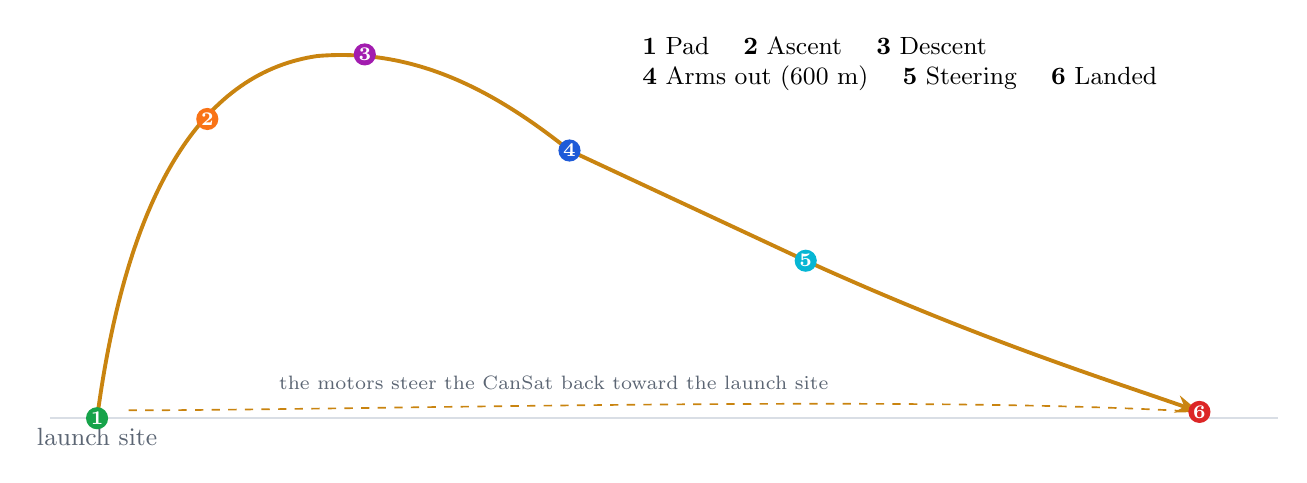
\begin{tikzpicture}[x=1cm,y=1cm,font=\small]
  \draw[rule,line width=0.6pt] (0,0) -- (15.6,0);
  \node[below,muted] at (0.6,0) {launch site};
  % path
  \draw[accent,line width=1.4pt,-{Stealth[length=3mm]}]
     (0.6,0) .. controls (1.0,3.0) and (2.0,4.4) .. (3.4,4.6)
     .. controls (4.6,4.7) and (5.6,4.2) .. (6.6,3.4)
     -- (9.6,2.0) .. controls (11.8,1.0) and (13.4,0.5) .. (14.6,0.08);
  \draw[accent,line width=0.6pt,dashed] (14.6,0.08) .. controls (11,0.3) and (4,0.1) .. (0.9,0.1);
  % markers
  \foreach \x/\y/\c/\t/\p in {0.6/0/ledgreen/1/below right,2.0/3.8/ledorange/2/left,4.0/4.62/ledpurple/3/above,
                              6.6/3.4/ledblue/4/above right,9.6/2.0/ledcyan/5/above right,14.6/0.08/ledred/6/above}
    {\fill[\c] (\x,\y) circle (4pt); \node[font=\scriptsize\bfseries,text=white] at (\x,\y) {\t};}
  \node[align=left,anchor=west] at (7.4,4.5) {\textbf{1} Pad \quad \textbf{2} Ascent \quad \textbf{3} Descent\\
       \textbf{4} Arms out (600 m) \quad \textbf{5} Steering \quad \textbf{6} Landed};
  \node[muted,font=\scriptsize] at (6.4,0.45) {the motors steer the CanSat back toward the launch site};
\end{tikzpicture}
\end{figure}

\begin{enumerate}
  \item \textbf{Pad.} It waits on the ground. It measures the air pressure (to know the
        launch-site height), finds its position with satellites, and works out how it is mounted.
  \item \textbf{Ascent.} It notices that it is being carried up.
  \item \textbf{Descent.} It notices that it has been released. The parachute opens by itself.
  \item \textbf{Arms out.} At \textbf{600 metres} above the launch site, two small servos unlock
        the four drone arms, which fold out.
  \item \textbf{Steering.} The four motors start. They tilt the CanSat under its parachute and push it
        back toward the launch site. They stop 10 metres above the ground.
  \item \textbf{Landed.} It switches the motors off for good, blinks red and beeps so you can find it.
\end{enumerate}

During the whole flight it records its data internally, about one hour's worth. If radio telemetry
is switched on, it also sends one data line per second to the ground station.

\begin{good}
If the CanSat restarts in the air (for example after a loose battery contact), it remembers where
it was in the mission and carries on. It does not start again from ``Pad''.
\end{good}

% =============================================================================
\section{Safety}

\begin{danger}[Propellers]
\begin{itemize}[leftmargin=12pt]
  \item Bench work, motor tests, servo tests: \textbf{propellers off}.
  \item The motors can only spin when the battery is connected. USB alone cannot spin them.
  \item In flight the motors stop by themselves at 10 m above the ground. During a lift test
        they are locked off completely.
  \item If anything looks wrong while motors are running, press \btn{Abort motors} (Bench page) or
        type \cmd{CMD,001,ABORT} in the Console. The motors then stay off for the rest of the flight.
\end{itemize}
\end{danger}

\begin{danger}[Battery]
Use only the 2-cell Li-ion pack supplied with the CanSat. Do not charge it unattended, do not use
it if it is swollen or damaged, and disconnect it when you are not using the CanSat.
\end{danger}

% =============================================================================
\section{What you need}

\begin{tabularx}{\linewidth}{@{}lL@{}}
\toprule
\textbf{Item} & \textbf{Notes} \\ \midrule
The CanSat & With the flight computer inside (an ESP32-S3 board with a small multi-colour light) \\
Charged battery & 2-cell Li-ion pack (only needed for motors, servos and flight) \\
USB-C data cable & Some cables only charge. If the laptop does not see the CanSat, try another cable \\
Windows laptop & With Bluetooth (most laptops have it) and the \texttt{cansat\_fw} folder \\
Phone with a compass app & Only for the one-time north calibration \\
Ground radio (XBee) & Only if the radio is fitted in the CanSat; plugs into the laptop by USB \\
\bottomrule
\end{tabularx}

% =============================================================================
\section{Setting up the laptop (one time)}\label{sec:setup}

\begin{enumerate}
  \item \textbf{Install Python.} Go to \url{https://www.python.org/downloads/}, download the
        latest Python for Windows and run the installer. On the first screen tick
        \textbf{``Add python.exe to PATH''}, then click \emph{Install Now}.
  \item \textbf{Get the CanSat folder.} Copy the \texttt{cansat\_fw} folder to the laptop
        (from a USB stick, or from GitHub with \emph{Code → Download ZIP} and then \emph{Extract all}).
        Put it somewhere easy to find, such as the Desktop.
  \item \textbf{Start the ground station.} Open the folder and double-click
        \textbf{\texttt{LAUNCH\_DOCK.bat}}. The first time, a black window appears and installs the
        packages it needs (internet required, about a minute). After that the ground station
        (we call it \emph{the dock}) opens.
\end{enumerate}

\begin{tip}
If Windows shows ``Windows protected your PC'', click \emph{More info → Run anyway}. The file
only starts the dock. To make a desktop shortcut, right-click \texttt{LAUNCH\_DOCK.bat} and choose
\emph{Send to → Desktop (create shortcut)}.
\end{tip}

% =============================================================================
\section{Switching the CanSat on}\label{sec:poweron}

The CanSat switches on as soon as it gets power: either the USB cable from the laptop, or the
battery. There is no on/off button.

\begin{tip}[Important]
Switch it on \textbf{standing upright and keep it still} for the first few seconds. This is when
it works out how it is mounted and measures the launch-site air pressure.
\end{tip}

\subsection{The start-up light}\label{sec:led}

Watch the small multi-colour light on the flight computer. It goes through this sequence:

\begin{center}
\renewcommand{\arraystretch}{1.35}
\begin{tabularx}{\linewidth}{@{}c l L@{}}
\toprule
& \textbf{Light} & \textbf{Meaning} \\ \midrule
\led{ledwhite}\,\led{ledblue} & White, then blue & Powering up, starting the sensors \\
\led{ledviolet} & Violet, slowly breathing & Finding its orientation: \textbf{keep it still} \\
\led{ledgreen}\,\led{ledgreen} & Two green blinks & \textbf{All checks passed} \\
\led{ledamber}\,\led{ledamber} & Two amber blinks & Passed with warnings: an optional part is missing (normal at the moment, see below) \\
\led{ledred}\,\led{ledred}\,\led{ledred} & Three red blinks & A main sensor is missing. \textbf{Do not fly}; see Troubleshooting \\
\led{ledmagenta} & One magenta flash & It restarted in the air and is carrying on with the mission \\
\bottomrule
\end{tabularx}
\end{center}

After the start-up sequence, the light shows the mission phase:

\begin{center}
\renewcommand{\arraystretch}{1.35}
\begin{tabularx}{\linewidth}{@{}c l L@{}}
\toprule
& \textbf{Colour} & \textbf{Phase} \\ \midrule
\led{ledgreen} & Green & Pad: waiting on the ground \\
\led{ledorange} & Orange & Ascent: being carried up \\
\led{ledpurple} & Purple & Descent: released, under the parachute \\
\led{ledblue} & Blue & Arms out \\
\led{ledcyan} & Cyan & Steering with the motors \\
\led{ledred} & Blinking red + beeping & Landed: come and find me \\
\bottomrule
\end{tabularx}
\end{center}

\begin{good}[Why amber is normal right now]
Some parts (battery monitor, SD card) are not fitted yet. The CanSat reports them as missing,
which gives two amber blinks. The \page{Health} page in the dock tells you exactly which parts.
Red is the colour to worry about.
\end{good}

% =============================================================================
\section{Connecting the dock to the CanSat}\label{sec:connect}

The dock can talk to the CanSat in two ways:

\begin{tabularx}{\linewidth}{@{}lL@{}}
\toprule
\textbf{USB cable} & Everything works: live data, health, downloading the flight log, motor and servo tests, firmware updates. \\
\textbf{Bluetooth} & Wireless check-ups from a few metres away: live data, health, calibration, simulated flights. Motor and servo tests, log download and erasing are blocked over Bluetooth for safety. \\
\bottomrule
\end{tabularx}

\subsection{Over USB}
\begin{enumerate}
  \item Plug the USB cable into the CanSat's USB port and into the laptop.
  \item In the dock's top bar, click \btn{USB}.
  \item Pick the port in the list (it usually shows up as \texttt{COM} and a number). If you are
        not sure, unplug the cable, press the refresh button, plug it back in and see which one appears.
  \item Click \btn{Connect}. The dot next to the port turns green and the numbers start moving.
\end{enumerate}

\subsection{Over Bluetooth}
\begin{enumerate}
  \item Make sure Bluetooth is switched on in Windows (\emph{Settings → Bluetooth \& devices}).
        You do \emph{not} need to pair the CanSat in Windows.
  \item In the dock's top bar, click \btn{Bluetooth}, then \btn{Connect}.
  \item The dock looks for a CanSat called \textbf{AAKASHVANI-001} and connects. The top bar
        then shows ``Bluetooth AAKASHVANI-001''.
\end{enumerate}

\shot[0.92\linewidth]{ble_health.png}{The dock connected over Bluetooth (top right), showing the Health page.}

\begin{good}
Bluetooth switches itself off when a real flight starts, so it cannot interfere with the radio.
It switches back on after landing, which lets you check the CanSat without opening it.
\end{good}

% =============================================================================
\section{The dock, page by page}

The pages are listed on the left. The bar along the bottom shows the time since the CanSat was
switched on, how many data packets have arrived, and whether the ground telemetry file is being
recorded.

\subsection{Overview}
\shot[0.92\linewidth]{overview.png}{Overview page on the pad.}
\begin{itemize}
  \item \textbf{Phase rail} (top): the six phases. The current one is highlighted.
  \item \textbf{Altitude above pad}, \textbf{Vertical speed} (negative = going down),
        \textbf{Peak} (highest point so far) and \textbf{Time since power-on}.
  \item \textbf{Altitude chart}: the last two minutes.
  \item \textbf{Return to launch}: distance and direction to the launch site, satellites in view,
        how much the CanSat is being tilted, whether the drone arms are latched, and whether the motors are running.
        ``no site fix'' means it has not yet seen enough satellites to know where the launch site is.
  \item \textbf{Events}: a running list of what happened (launch, release, arms out, landed …).
\end{itemize}

\subsection{Attitude}
\shot[0.92\linewidth]{attitude.png}{Attitude page.}
Shows how the CanSat is tilted (\emph{pitch} and \emph{roll}) and which way it is pointing (\emph{heading}).
Tilt the CanSat by hand and watch the horizon move.
\begin{itemize}
  \item \btn{3D view} / \btn{3D view in browser}: a 3D model of the CanSat that moves with the real one.
  \item \btn{Re-reference}: tells the CanSat that its current position is ``upright''. Use it after you
        move the flight computer inside the CanSat. Only works on the pad.
  \item \btn{Calibrate north}: see Section~\ref{sec:north}.
\end{itemize}

\shot[0.92\linewidth]{viewer_live.png}{The 3D view in the browser. Use the buttons on the left to change the camera, the shell transparency and the exploded view.}

\subsection{Health}
\shot[0.92\linewidth]{health.png}{Health page. A green dot means good, amber means attention, grey means not fitted.}
The quick check before every flight:

\begin{tabularx}{\linewidth}{@{}lL@{}}
\toprule
\textbf{Card} & \textbf{What you want to see} \\ \midrule
IMU & About 100 Hz. The small text shows how the sensor is mounted \\
Barometer & OK \\
GNSS & 5 or more satellites (outdoors, after a minute or two) \\
Battery & The voltage once the battery monitor is fitted; ``not fitted'' until then \\
Free memory & Above about 100 KB \\
Flight log & ``3.0 MB pre-erased ahead''. This needs about 2 minutes after switching on \\
Bluetooth & Advertising (waiting) or Connected \\
Self test & Which optional parts are missing; whether a crash report is stored \\
\bottomrule
\end{tabularx}

\subsection{Flight log}
\shot[0.92\linewidth]{log_list.png}{Flight log page with the list of recorded sessions.}
Two different things live here:
\begin{itemize}
  \item \textbf{Ground telemetry file (for the judges).} Every data line the dock receives is saved to
        \judgesfile{}.
        \btn{Open folder} shows it. \btn{Start fresh file} renames the old file (adding the date) and starts a new one.
  \item \textbf{On-board recorder sessions.} Each time the CanSat is switched on, it records a new session
        inside its own memory. \btn{Refresh list} reads the list, \btn{Download selected} saves the chosen
        session to the laptop as a spreadsheet file (CSV), \btn{Crash report} shows details if the software ever
        crashed, and \btn{Erase log} deletes all sessions. USB only.
\end{itemize}
When the memory is full, the oldest data is overwritten. A session whose beginning has been
overwritten shows as ``start overwritten''.

\subsection{Bench}
\shot[0.92\linewidth]{bench.png}{Bench page.}
\begin{itemize}
  \item \btn{Zero altitude}: makes the current height the launch-site height and puts the mission back to ``Pad''.
        Use it if you moved the CanSat to a different floor or place after switching on.
  \item \btn{Reset mission clock}: sets the mission clock to 00:00:00.
  \item \textbf{Radio telemetry (CX)}: switches the radio data link on or off. It is \emph{off} every
        time the CanSat starts; the competition rules say the CanSat must not transmit until you are
        told to start.
  \item \textbf{Lift test}: see Section~\ref{sec:lift}.
  \item \textbf{Simulated flight}: see Section~\ref{sec:sim}.
  \item \textbf{Actuators (props off)}: spin one motor (\btn{M1}…\btn{M4}) or \btn{All} for 3 seconds at the
        throttle you set, open the arm latches, or \btn{Abort motors}. USB only, propellers off.
\end{itemize}

\subsection{Console}
\shot[0.85\linewidth]{console.png}{Console page: the raw lines from the CanSat.}
For advanced use. You can type commands such as \cmd{CMD,001,LOG,LIST} and press Enter.
Appendix~\ref{sec:commands} lists them. You will not normally need this page.

\subsection{Firmware}
\shot[0.85\linewidth]{firmware.png}{Firmware page.}
Puts new software on the CanSat. See Section~\ref{sec:update}.

% =============================================================================
\section{Flight day, step by step}\label{sec:flightday}

\subsection{The day before}
\begin{enumerate}
  \item Charge the battery.
  \item Connect over USB, open \page{Flight log}, and download any session you want to keep.
  \item On \page{Flight log}, click \btn{Start fresh file}, so the judges' file contains only flight day.
  \item If the flight computer was moved or remounted: do the north calibration (\ref{sec:north}).
\end{enumerate}

\subsection{At the launch site}
\begin{enumerate}
  \item Start the dock on the laptop.
  \item Stand the CanSat \textbf{upright on the ground}, connect the battery (propellers on only if flying now)
        and \textbf{keep it still} until the light has finished its start-up sequence.
  \item Check the light: two green or two amber blinks, then steady green.
  \item Connect the dock (USB or Bluetooth).
  \item \page{Overview}: phase \textbf{Pad}, altitude close to 0 m.
  \item \page{Health}: IMU about 100 Hz, barometer OK, GNSS 5+ satellites, flight log 3.0 MB pre-erased.
  \item \page{Overview} → Return to launch: the distance to the site shows a number (not ``no site fix'').
        This needs 5+ satellites for about 10 seconds.
  \item If you used USB, unplug it now. The CanSat keeps running on its battery.
  \item When the judges say radio transmission may start: \page{Bench} → switch on
        \textbf{Radio telemetry (CX)}.
  \item Check that the status bar shows ``recording Flight\_2026-IN-SPACeCAN-7USAT-001.csv'' with the row count increasing.
\end{enumerate}

\begin{tip}
Switch the CanSat on at least \textbf{2 minutes before launch}. It uses this time to prepare its
internal memory for the flight recording.
\end{tip}

\subsection{During the flight}
You do not need to do anything. On the \page{Overview} page you will see the phases light up one by
one, and the events list will fill. Keep the dock running so the judges' file keeps recording.

Only if the motors behave dangerously: press \btn{Abort motors} (needs a working radio link).

\subsection{After landing}
\begin{enumerate}
  \item Follow the beeping and the blinking red light to find the CanSat.
  \item Disconnect the battery (keep away from the propellers).
  \item Hand in \judgesfile{}
        (\page{Flight log} → \btn{Open folder}).
  \item Back at the table, connect USB, open \page{Flight log}, \btn{Refresh list}, select the newest session
        (\#1) and \btn{Download selected}. This is the detailed recording (50 lines per second) for later analysis.
\end{enumerate}

% =============================================================================
\section{Practising without flying}

\subsection{Simulated flight (on the table)}\label{sec:sim}
The dock feeds the CanSat a pretend flight, and the CanSat reacts exactly as it would in the air.
\begin{enumerate}
  \item Connect (USB or Bluetooth). Propellers off.
  \item \page{Bench} → Simulated flight → choose \emph{Carrier drone to 750 m} → \btn{Run}.
  \item Switch to \page{Overview} and watch: Pad → Ascent → Descent → Arms out (at 600 m) → Steering → Landed.
        It takes about two minutes. If the servos are connected, you will hear them unlock.
  \item At the end, click \btn{Zero altitude} on the Bench page to return to Pad.
\end{enumerate}

\subsection{Lift (elevator) test, with real sensors}\label{sec:lift}
This shows the whole sequence at the size of a building, using the real sensors. The motors
are locked off for the whole test.
\begin{enumerate}
  \item On the ground floor: \page{Bench} → Lift test → ``Open arms at'' \textbf{10} m → \btn{Start}.
  \item Ride up at least 4 floors (the phase becomes Ascent), then ride back down.
  \item Shortly after you start going down: Descent. 10 m above the start floor: Arms out (the servos unlock).
        At the bottom: Landed.
  \item \btn{Zero altitude} for another ride, or \btn{Stop} to end the test. Switching the CanSat off and on
        also ends it.
\end{enumerate}

% =============================================================================
\section{One-time calibrations}

\subsection{North calibration}\label{sec:north}
The CanSat needs to know true north to steer home. Do this once, and again whenever the flight
computer is remounted.
\begin{enumerate}
  \item Open a compass app on your phone, away from metal and electronics.
  \item Point the CanSat's front (its \emph{+X} side; ask the team to mark it on the shell) at north and hold it still.
  \item \page{Attitude} → \btn{Calibrate north} → OK. The setting is stored in the CanSat.
\end{enumerate}

% =============================================================================
\section{Updating the software}\label{sec:update}
Only needed when the team gives you a new version. It always uses the USB cable; wireless updates
are not possible.
\begin{enumerate}
  \item Make sure the new software has been built (the team does this; the folder \texttt{build} then contains it).
  \item Connect over USB.
  \item \page{Firmware} → \btn{Flash firmware}. Wait until the window says ``Done.'' (about 30 seconds).
  \item The CanSat restarts and plays its start-up light. Click \btn{Connect} again.
\end{enumerate}
Updating keeps the settings, the flight recordings and the crash report.
\btn{Erase entire flash} deletes \emph{everything}, including the recordings. Do not use it unless told to.

% =============================================================================
\clearpage
\section{Troubleshooting}

\renewcommand{\arraystretch}{1.3}
\begin{tabularx}{\linewidth}{@{}>{\raggedright\arraybackslash}p{0.33\linewidth}L@{}}
\toprule
\textbf{Problem} & \textbf{What to do} \\ \midrule
No light at all & Check the battery is charged and connected, or try the USB cable in another port. \\
Three red blinks & A main sensor (orientation or pressure) did not answer. Switch off, check that the sensor board is firmly connected, switch on again. If it persists, do not fly; tell the team. \\
Two amber blinks & Usually normal (optional parts not fitted). Check \page{Health} → Self test for the list. \\
No COM port in the list & Use a different USB cable (some only charge). Press the refresh button next to the list. \\
``Connect'' over USB does nothing & Close any other program that might use the port (Arduino, another dock window), then try again. \\
Bluetooth does not find AAKASHVANI-001 & Switch Bluetooth on in Windows. Move closer. The CanSat turns Bluetooth off during a flight and back on after landing; switch it off and on again if it is stuck in a flight phase. \\
``That command needs the USB link'' & Motor and servo tests, log download and erase are blocked over Bluetooth. Connect the cable. \\
GNSS shows 0 satellites & Go outdoors with a clear view of the sky and wait 2–5 minutes. Indoors it will not find satellites. \\
``no site fix'' on Overview & It needs 5+ satellites for about 10 seconds. If you moved, click \btn{Zero altitude} after the fix. \\
Altitude is not 0 on the pad & Click \btn{Zero altitude} on the Bench page. \\
Phase is not ``Pad'' before flight & Click \btn{Zero altitude}; it also resets the mission to Pad. \\
The 3D view stays still & Check that the dock is connected. In the browser view, click \emph{Live} in the left panel. \\
Flight log list is empty & Wait a few seconds after \btn{Refresh list}; reading 12 MB takes about 2 seconds. It needs USB. \\
``Crash dump stored'' on Health & The software crashed at some point. Click \btn{Crash report} on the Flight log page and send the text to the team. \\
Dock window closes with an error & Run \texttt{LAUNCH\_DOCK.bat} again and read the message in the black window. Check that the internet was available on the first start. \\
\bottomrule
\end{tabularx}

% =============================================================================
\needspace{16\baselineskip}
\section{Words used in this manual}

\begin{tabularx}{\linewidth}{@{}lL@{}}
\toprule
AGL & ``Above ground level'': height above the launch site. \\
Attitude & How the CanSat is tilted and turned. \\
Barometer & The pressure sensor that measures height. \\
Dock & The ground-station program on the laptop. \\
Firmware & The software inside the CanSat. \\
GNSS & Satellite navigation (GPS and India's NavIC). \\
Heading & The compass direction the CanSat faces. \\
IMU & The orientation sensor (it measures tilt, turning and acceleration). \\
Pitch / roll & Tilt forward/backward and tilt sideways. \\
Servo & A small motor that moves to a set position; here it unlocks the drone arms. \\
Telemetry & Data the CanSat sends to the ground while it flies. \\
\bottomrule
\end{tabularx}

% =============================================================================
\appendix
\section{Quick reference}\label{sec:quickref}

\begin{minipage}[t]{0.48\linewidth}
\textbf{Start-up light}\par\smallskip
\renewcommand{\arraystretch}{1.3}
\begin{tabular}{@{}c l@{}}
\led{ledwhite}\,\led{ledblue} & powering up \\
\led{ledviolet} & orienting: keep still \\
\led{ledgreen}\,\led{ledgreen} & all good \\
\led{ledamber}\,\led{ledamber} & good, optional part missing \\
\led{ledred}\,\led{ledred}\,\led{ledred} & main sensor missing: no flight \\
\led{ledmagenta} & restarted in the air \\
\end{tabular}
\end{minipage}\hfill
\begin{minipage}[t]{0.48\linewidth}
\textbf{Phase colours}\par\smallskip
\renewcommand{\arraystretch}{1.3}
\begin{tabular}{@{}c l@{}}
\led{ledgreen} & Pad \\
\led{ledorange} & Ascent \\
\led{ledpurple} & Descent (parachute) \\
\led{ledblue} & Arms out (600 m) \\
\led{ledcyan} & Steering \\
\led{ledred} & Landed (blinking, beeping) \\
\end{tabular}
\end{minipage}

\bigskip
\textbf{Pre-launch in one line}: upright and still at switch-on → green/amber blinks → Pad, 0 m →
5+ satellites, site fix → 3.0 MB pre-erased → radio on when allowed → recording.

\bigskip
\textbf{The judges' file}: \judgesfile{}

\needspace{18\baselineskip}
\section{Console commands}\label{sec:commands}
Type in the \page{Console} page, then press Enter. All commands start with \cmd{CMD,001,}.

\renewcommand{\arraystretch}{1.25}
\begin{tabularx}{\linewidth}{@{}>{\ttfamily\raggedright\arraybackslash}p{0.36\linewidth}L@{}}
\toprule
\textrm{\textbf{Command}} & \textbf{What it does} \\ \midrule
CMD,001,CX,ON / CX,OFF & Radio telemetry on / off \\
CMD,001,CAL & Zero altitude, mission back to Pad \\
CMD,001,ST,00:00:00 & Set the mission clock \\
CMD,001,TARE & Re-reference ``upright'' (pad only) \\
CMD,001,NORTH & North calibration (pad only) \\
CMD,001,LIFT,10 / LIFT,OFF & Lift test on (arms at 10 m) / off \\
CMD,001,LOG,LIST & List recorded sessions \\
CMD,001,LOG,CRASH & Show the crash report \\
CMD,001,ABORT & Motors off for the rest of the flight \\
CMD,001,CHUTE & Open the arm latches now (USB) \\
CMD,001,MTR,0,8 & Spin motor 1 at 8\,\% for 3 s (USB, props off) \\
\bottomrule
\end{tabularx}

\end{document}
